\documentclass{article}

\usepackage{fancyhdr}
\usepackage{extramarks}
\usepackage{amsmath}
\usepackage{amsthm}
\usepackage{amsfonts}
\usepackage{tikz}
\usepackage[plain]{algorithm}
\usepackage{algpseudocode}
\usepackage{wrapfig}

\usetikzlibrary{automata,positioning}

%
% Basic Document Settings
%

\topmargin=-0.45in
\evensidemargin=0in
\oddsidemargin=0in
\textwidth=6.5in
\textheight=9.0in
\headsep=0.25in

\linespread{1.1}

\pagestyle{fancy}
\lhead{\hmwkAuthorName}
\rhead{\firstxmark}
\lfoot{\lastxmark}
\cfoot{\thepage}

\renewcommand\headrulewidth{0.4pt}
\renewcommand\footrulewidth{0.4pt}

\setlength\parindent{0pt}

%
% Create Problem Sections
%

\newcommand{\enterProblemHeader}[1]{
    \nobreak\extramarks{}{Problem \arabic{#1} continued on next page\ldots}\nobreak{}
    \nobreak\extramarks{Problem \arabic{#1} (continued)}{Problem \arabic{#1} continued on next page\ldots}\nobreak{}
}

\newcommand{\exitProblemHeader}[1]{
    \nobreak\extramarks{Problem \arabic{#1} (continued)}{Problem \arabic{#1} continued on next page\ldots}\nobreak{}
    \stepcounter{#1}
    \nobreak\extramarks{Problem \arabic{#1}}{}\nobreak{}
}

\setcounter{secnumdepth}{0}
\newcounter{partCounter}
\newcounter{homeworkProblemCounter}
\setcounter{homeworkProblemCounter}{1}
\nobreak\extramarks{Problem \arabic{homeworkProblemCounter}}{}\nobreak{}

%
% Homework Problem Environment
%
% This environment takes an optional argument. When given, it will adjust the
% problem counter. This is useful for when the problems given for your
% assignment aren't sequential. See the last 3 problems of this template for an
% example.
%
\newenvironment{homeworkProblem}[1][-1]{
    \ifnum#1>0
        \setcounter{homeworkProblemCounter}{#1}
    \fi
    \section{Problem \arabic{homeworkProblemCounter}}
    \setcounter{partCounter}{1}
    \enterProblemHeader{homeworkProblemCounter}
}{
    \exitProblemHeader{homeworkProblemCounter}
}

%
% Homework Details
%   - Title
%   - Due date
%   - Class
%   - Section/Time
%   - Instructor
%   - Author
%

\newcommand{\hmwkTitle}{Computer Assignment\ \#4}
\newcommand{\hmwkDueDate}{May 26, 2023}
\newcommand{\hmwkClass}{Natural Language Processing}
\newcommand{\hmwkClassTime}{Chapters 10, 11}
\newcommand{\hmwkClassInstructor}{Professor Hesham Faili}
\newcommand{\hmwkAuthorName}{\textbf{Tohid Abdi}}

%
% Title Page
%

\title{
    \vspace{2in}
    \textmd{\textbf{\hmwkClass:\ \hmwkTitle}}\\
    \normalsize\vspace{0.1in}\small{Due\ on\ \hmwkDueDate}\\
    \vspace{3in}
}

\author{\hmwkAuthorName}
\date{}

\renewcommand{\part}[1]{\textbf{\large Part \Alph{partCounter}}\stepcounter{partCounter}\\}

%
% Various Helper Commands
%

% Useful for algorithms
\newcommand{\alg}[1]{\textsc{\bfseries \footnotesize #1}}

% For derivatives
\newcommand{\deriv}[1]{\frac{\mathrm{d}}{\mathrm{d}x} (#1)}

% For partial derivatives
\newcommand{\pderiv}[2]{\frac{\partial}{\partial #1} (#2)}

% Integral dx
\newcommand{\dx}{\mathrm{d}x}

% Alias for the Solution section header
\newcommand{\solution}{\textbf{\large Solution}}

% Probability commands: Expectation, Variance, Covariance, Bias
\newcommand{\E}{\mathrm{E}}
\newcommand{\Var}{\mathrm{Var}}
\newcommand{\Cov}{\mathrm{Cov}}
\newcommand{\Bias}{\mathrm{Bias}}

\begin{document}

\maketitle

\pagebreak

\begin{homeworkProblem}

    \textbf{Dataset and Preprocessing.}


In the first step, we install and import the required libraries. We download and read the training, validation and test data through the GitHub link. In order to be able to use labels for model training, we use label encoding and map them to numbers from 0 to 2.\\

Distribution of labels for the training data is shown in Figure 1.

\begin{figure}
    \centering
    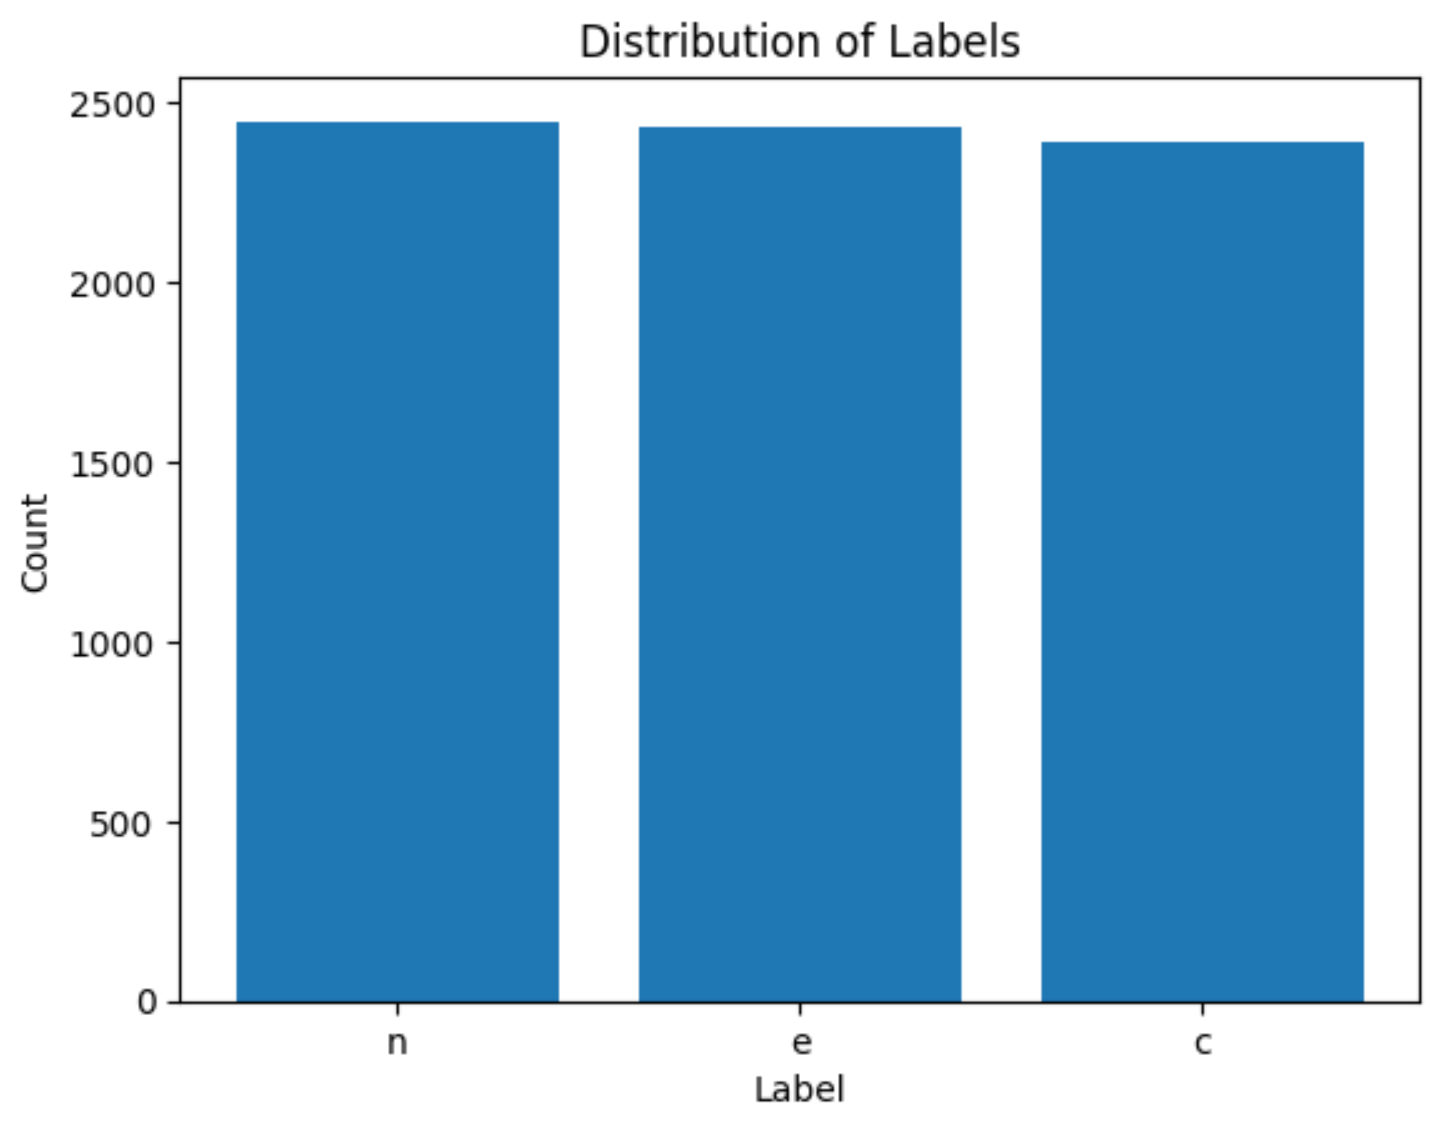
\includegraphics[width=0.5\textwidth]{1-1.png}
    \caption{Distribution of labels for Farstail dataset}
    \end{figure}
    
In the next step, we use the Re library to clean the text. Due to the fact that the Parsbert tokenizer performs the necessary pre-processing, we do not perform other pre-processings manually. Finally, we convert the data into Huggingface dataset.\\

    \textbf{Task 1.}
    
We download Tokenizer and Parsbert model from Huggingface. By applying padding with a maximum length of 192, we tokenize the sentences.\\

To build the model, we consider input ids, token type ids, and attention mask as inputs and to use Parsbert embedding, we take the output of the first hidden state and give it to the encoder transformer. With the help of average pooling and then feedforward layers, we obtain the output of the model. To train this model, we freeze Parsbert layer. We compile and train the model with Categorical Cross Entropy loss function and Adam optimizer.\\

After training the model for 30 epochs, the accuracy of the model on the test data is 0.7.\\

    \textbf{Task 2.}
    
We download Parsbert model with configuration of 3 labels for output and 3 hidden layers. The reason for using 3 hidden layers is to reduce the number of parameters and ease of comparison with the Task 1 model. With Sparse Categorical Cross-Entropy loss function and Adam optimizer, we compile the model and fine-tune it on Farstail data. Tables 1 and 2 show the evaluation of this model on the test data, and Figures 2 and 3 shows the loss and accuracy plots on the training and validation data.\\

\begin{table}
    \centering
    \caption{Evaluation of model for test data of Farstail dataset\\}   \begin{tabular}{|c|c|c|c|}
        \hline
        Accuracy & Precision & Recall & F1-score  \\ \hline
        0.4552 & 0.4552 & 0.4552 & 0.4552\\
        \hline
    \end{tabular}
\end{table}

\begin{table}
    \centering
    \caption{Confusion Matrix for Model for test data of Farstail dataset\\}   \begin{tabular}{|c|ccc|}
        \hline
        - & Actual n & Actual e & Actual c\\ \hline
        Predicted n & \textbf{219} & 157 & 123\\
        Predicted e & 159 & \textbf{239} & 158\\
        Predicted c & 132 & 123 & \textbf{254}\\
 \hline
    \end{tabular}
\end{table}

\begin{figure}
    \centering
    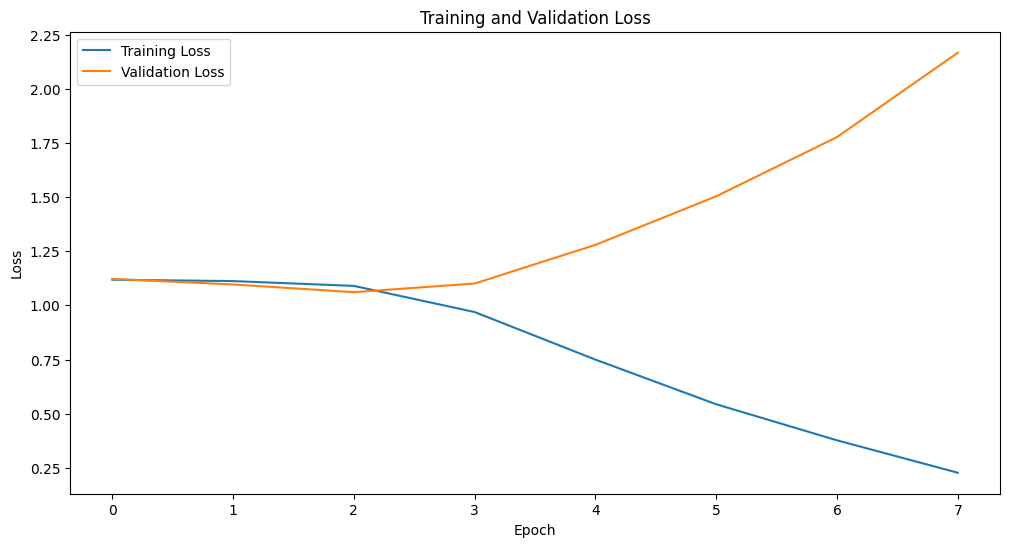
\includegraphics[width=0.5\textwidth]{1-3-1.png}
    \caption{Loss and Validation loss per epoch}
    \end{figure}
    
\begin{figure}
    \centering
    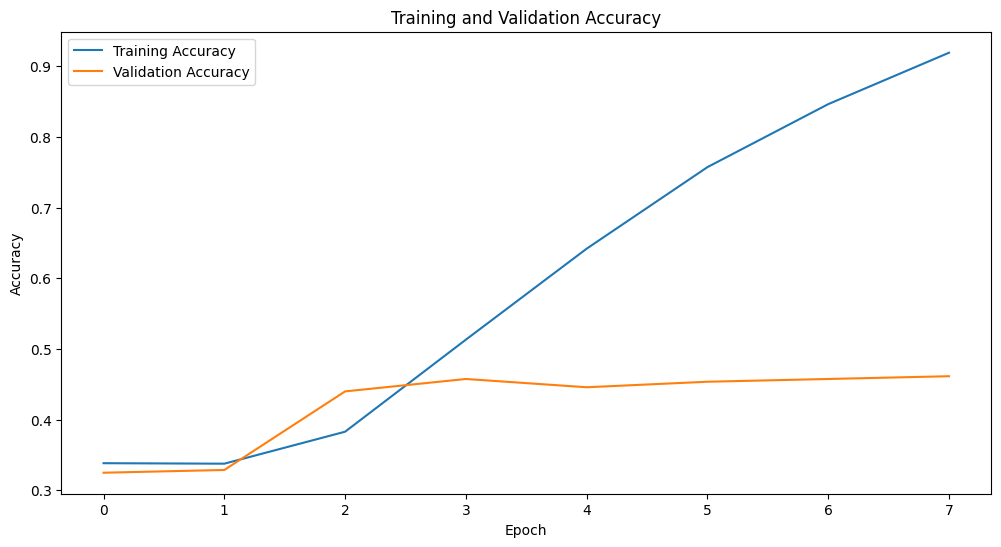
\includegraphics[width=0.5\textwidth]{1-3-2.png}
    \caption{Accuracy and Validation accuracy per epoch}
    \end{figure}
    
\pagebreak

    \textbf{Task 3.}
    
Figure 4 shows the accuracies plot for this task. Training data fine tuned for 1 epoch.\\

\begin{figure}
    \centering
    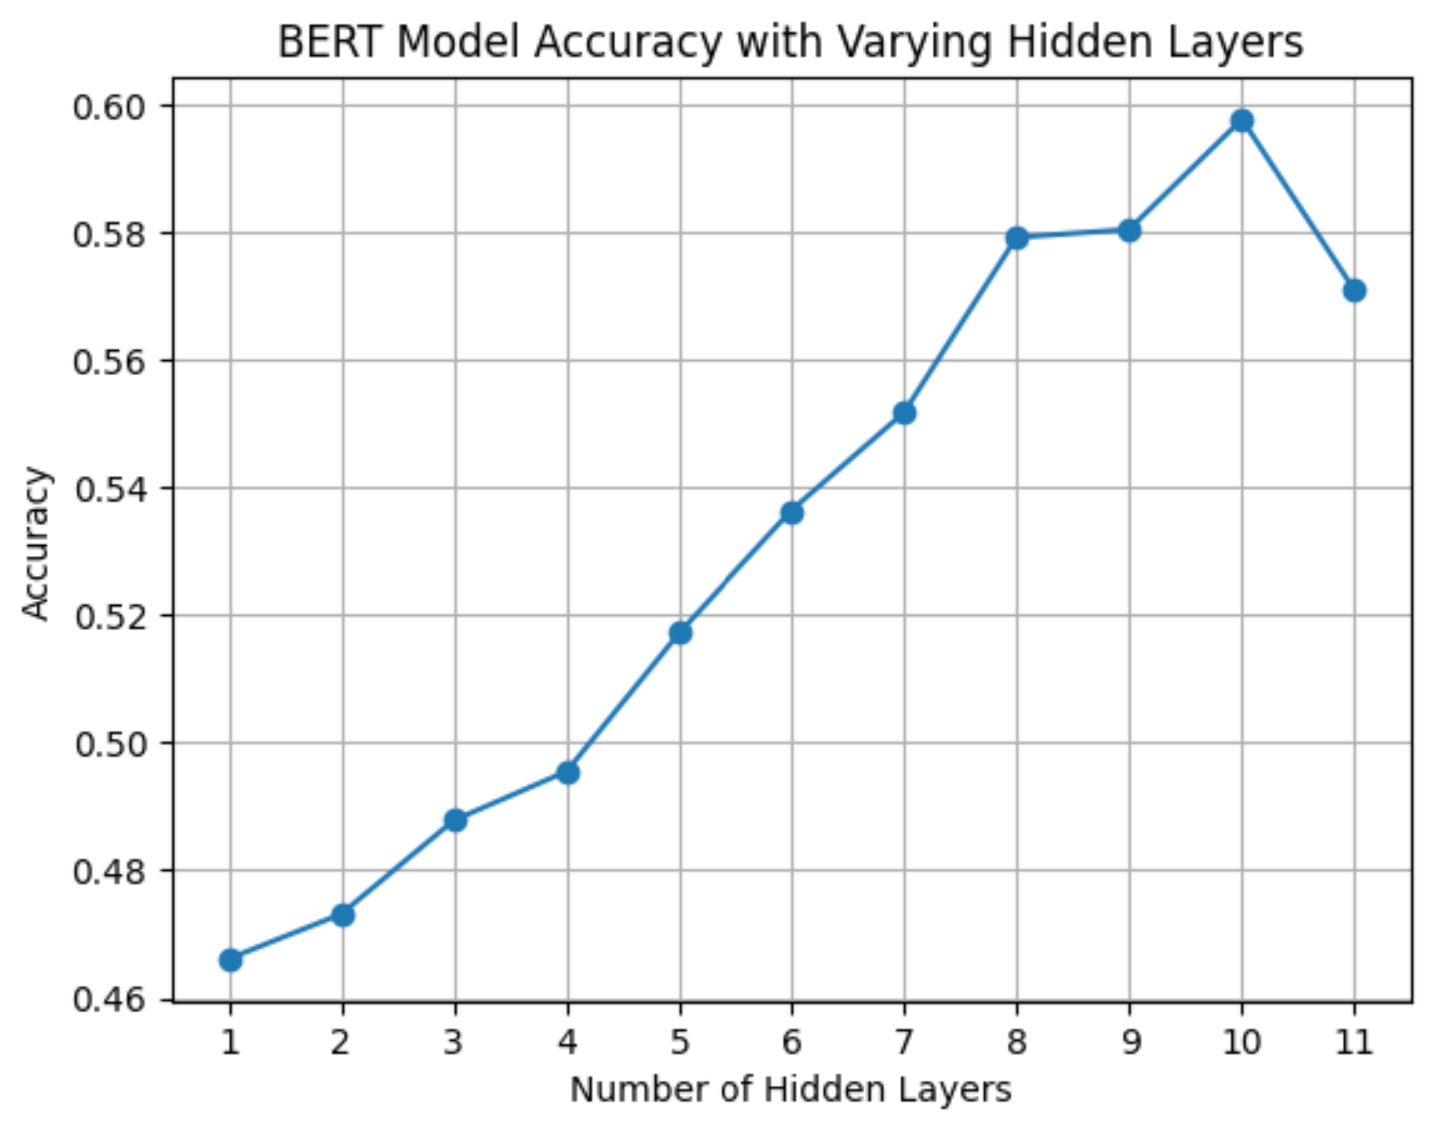
\includegraphics[width=0.5\textwidth]{1-4.png}
    \caption{Accuracy of test data for various number of hidden layers}
    \end{figure}
    
    \textbf{Task 4. \& 5.}
    
Done in notebook.\\

\pagebreak

\end{homeworkProblem}





\begin{homeworkProblem}



First of all,  we'll install the necessary Python packages. Then we import the necessary libraries which will be used in the notebook. In next step, we downloaded the Sentipers dataset.\\

    \textbf{1.}
    
We convert the 'polarity' column into numerical labels. Keeping the initial order, we divide the data into three categories: training, validation and testing. For ease of processing, we convert the text column of this data into tensorflow string. Figure 5 shows the distribution of labels for the polarity column.\\

\begin{figure}
    \centering
    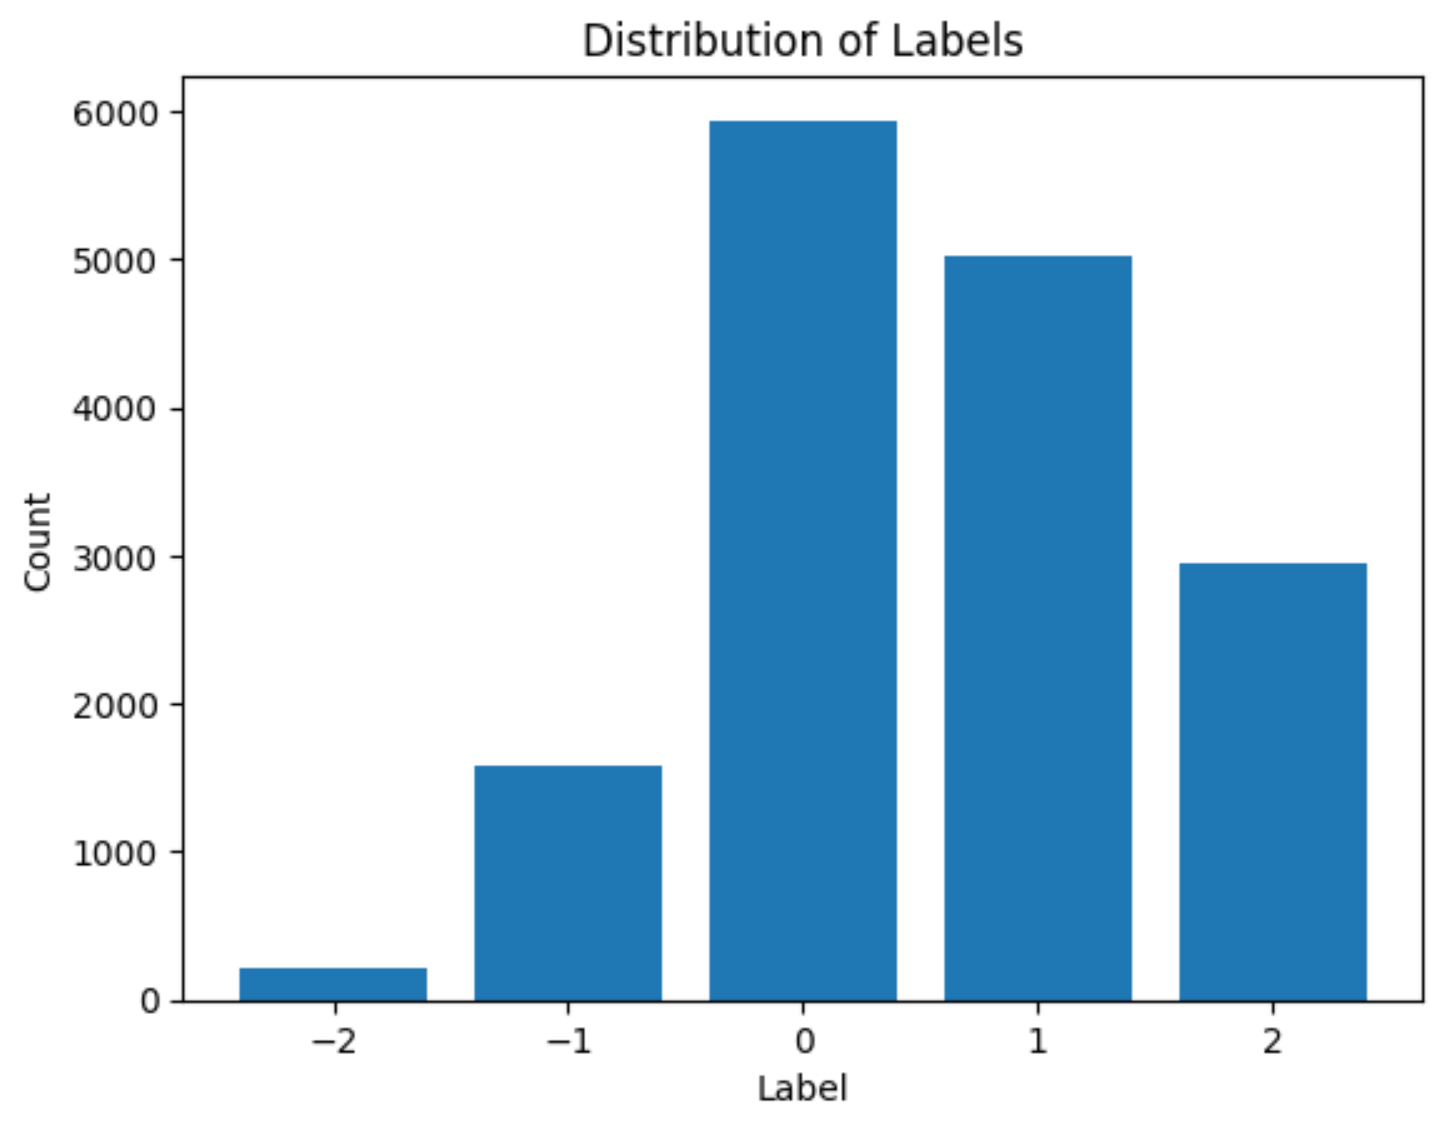
\includegraphics[width=0.5\textwidth]{2-1.png}
    \caption{Distribution of labels for the polarity column of Sentipers dataset}
    \end{figure}

    \textbf{2.}
    
In the first step, we download the pre-processing and encoder layers from Tensorhub. With a suitable architectural design, we prepare the model for fine-tuning. The input of the model will be in the form of text, this input enters the pre-processing layer and then passes through the encoder. After pooling and dropout, we have a linear layer with 5 neurons and a softmax activation function that determines the probability of the input belongig to each of the five classes.\\

We compile the model with cross entropy loss function and AdamW optimizer. We use early stop callback to determine the optimal number of epochs, and with a batch size of 32, we fine-tune the model for 20 epochs on Sentipers dataset.

    \textbf{3.}
    
The requested values for test data are shown in Table 3. This metrics are computed for classification of 5 classes.\\


\begin{table}
    \centering
    \caption{Evaluation of model for test data of Sentipers dataset\\}   \begin{tabular}{|c|c|c|c|}
        \hline
        Accuracy & Precision & Recall & F1-score  \\ \hline
        0.6246 & 0.6246 & 0.6246 & 0.6246\\
        \hline
    \end{tabular}
\end{table}

    \textbf{4.}

Table 4 shows the confusion matrix for Sentipers test data. The good performance of the model is evident in sentiment analysis.\\
      
\begin{table}
    \centering
    \caption{Confusion Matrix for Model for test data of Sentipers dataset\\}   \begin{tabular}{|c|ccccc|}
        \hline
        - & Actual -2 & Actual -1 & Actual 0 & Actual 1 & Actual 2  \\ \hline
        Predicted -2 & \textbf{0} & 1 & 0 & 0 & 0\\
        Predicted -1 & 6 & \textbf{61} & 23 & 16 & 4\\
        Predicted 0 & 6 & 39 & \textbf{447} & 181 & 15\\
        Predicted 1 & 4 & 22 & 73 & \textbf{300} & 84\\
        Predicted 2 & 2 & 4 & 7 & 102 & \textbf{172}\\
 \hline
    \end{tabular}
\end{table}

    \textbf{5.}

We import the data and map the labels to the values 0 and 1 and convert the comment column to the tensorflow string. To map the labels for zero-shot learning, we map the -2, -1 and 0 labels to 'sad' and 1 and 2 labels to 'happy'.\\

    \textbf{6.}
    
The requested values for snapfood test data are shown in Table 5. This metrics are computed for classification of 2 classes.\\


\begin{table}
    \centering
    \caption{Evaluation of model for test data of snapfood dataset\\}   \begin{tabular}{|c|c|c|c|}
        \hline
        Accuracy & Precision & Recall & F1-score  \\ \hline
        0.6964 & 0.6964 & 0.6964 & 0.6964\\
        \hline
    \end{tabular}
\end{table}


    \textbf{7.}
    
Table 6 shows the confusion matrix of the model, after zero-shot learning.\\
      
\begin{table}
    \centering
    \caption{Confusion Matrix for Model for test data of snapfood dataset\\}   \begin{tabular}{|c|cc|}
        \hline
        - & Actual sad & Actual happy\\ \hline
        Predicted sad & \textbf{1838} & 463\\
        Predicted happy & 1662 & \textbf{3037}\\
 \hline
    \end{tabular}
\end{table}

    \textbf{8.}
    
Zero-shot learning can be effective for sentiment analysis because it allows the model to generalize its understanding of sentiment across different domains or categories.\\

In this problem, model is trained on Sentipers data and this enables it to learn a general representation of sentiment. It learns to associate words, phrases, or patterns with positive or negative sentiment without relying on explicit domain-specific labels. This broader understanding of sentiment can then be applied to new domains such as snapfood dataset, even when that were not seen during training.\\

By employing zero-shot learning for sentiment analysis, we can overcome the limitations of traditional models that require domain-specific labeled data for each new task. It allows for more efficient and flexible sentiment analysis across a wide range of domains or categories, making it particularly useful in scenarios where the training data is limited, costly, or rapidly evolving.

\end{homeworkProblem}

\end{document}
